\documentclass[border=5mm]{standalone}
\usepackage{amsmath}
\usepackage{amssymb}
\usepackage{tikz}
\usetikzlibrary{arrows.meta,calc,shapes.geometric}

\definecolor{baselinefill}{HTML}{EAF4EA}
\definecolor{expfill}{HTML}{E8EEF6}
\definecolor{outfill}{HTML}{FFF5EB}
\definecolor{personA}{HTML}{0072B2}
\definecolor{personB}{HTML}{D55E00}
\definecolor{personC}{HTML}{009E73}
\definecolor{personD}{HTML}{882288}
\definecolor{shiftred}{HTML}{CC3333}

\begin{document}
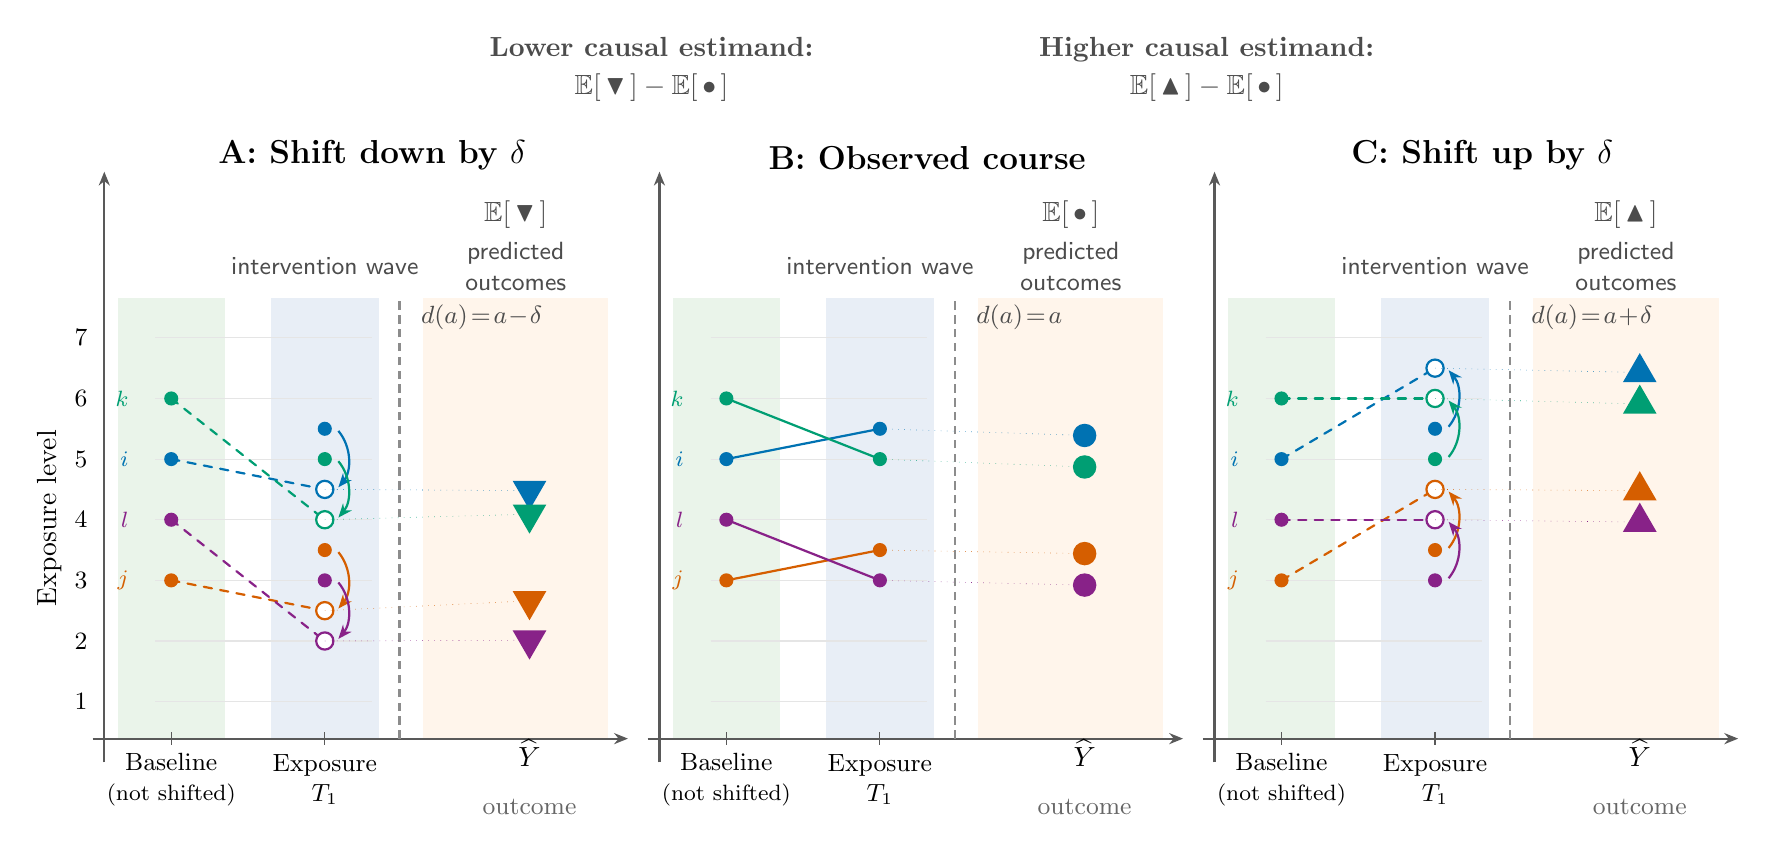
\begin{tikzpicture}[
  every node/.style={font=\normalsize, text=black},
  traj/.style={thick, line cap=round, line join=round},
  dot/.style={circle, inner sep=1.8pt, fill},
  ghost/.style={circle, inner sep=2.2pt, draw=#1, fill=white, line width=0.8pt},
  ghost/.default=black,
  connector/.style={very thin, dotted, black!30},
  shiftarrow/.style={-{Stealth[length=5pt, width=4pt]}, thick, shorten >=1pt, shorten <=1pt},
  outcome/.style={circle, inner sep=3.0pt, fill},
  outcome-down/.style={regular polygon, regular polygon sides=3, shape border rotate=180,
    inner sep=2.2pt, draw, thick, fill=white},
  outcome-up/.style={regular polygon, regular polygon sides=3,
    inner sep=2.2pt, draw, thick, fill=white},
  axis/.style={black!65, thick, -{Stealth[length=5pt, width=4pt]}}
]

\def\xs{1.95}
\def\ys{0.77}
\def\panelsep{7.05}
\def\outx{4.55}
\def\arrowxoff{0.15}
\def\outcol{4.375}  % centre of outcome column: (3.2+5.55)/2

\newcommand{\wx}[1]{\xs*#1}
\newcommand{\wy}[1]{\ys*#1}

% ============================================================
% PANEL A: SHIFT DOWN
% ============================================================
\begin{scope}[xshift=0cm]
  \fill[baselinefill] ({\wx{-0.35}},0.3) rectangle ({\wx{0.35}},5.9);
  \fill[expfill] ({\wx{0.65}},0.3) rectangle ({\wx{1.35}},5.9);
  \fill[outfill] (3.2,0.3) rectangle (5.55,5.9);

  \draw[axis] (-1.0,0.3) -- (5.8,0.3);
  \draw[axis] (-0.85,0.0) -- (-0.85,7.5);
  \draw[black!45, densely dashed, thick] (2.9,0.3) -- (2.9,5.9);

  \foreach \y in {1,2,3,4,5,6,7} {
    \draw[gray!20] (-0.2,{\wy{\y}}) -- (2.55,{\wy{\y}});
    \node[left, font=\small] at (-0.94,{\wy{\y}}) {\y};
  }

  \foreach \x in {0,1} {
    \draw[black!65] ({\wx{\x}},0.22) -- ({\wx{\x}},0.38);
  }

  \node[font=\small, align=center] at ({\wx{0}},-0.22) {Baseline\\{\footnotesize(not shifted)}};
  \node[font=\small, align=center] at ({\wx{1}},-0.22) {Exposure\\$T_1$};
  \node[font=\normalsize, anchor=base] at (\outx,-0.05) {$\widehat{Y}$};
  \node[font=\small, black!60, anchor=north] at (\outx,-0.35) {outcome};
  \node[rotate=90, font=\normalsize] at (-1.55,3.1) {Exposure level};

  % region labels
  \node[font=\sffamily\small, black!70] at ({\wx{1}},6.3) {intervention wave};
  \node[font=\sffamily\small, black!70, text width=1.5cm, align=center] at (\outcol,6.3) {predicted\\outcomes};

  % E[symbol] label
  \node[font=\normalsize\bfseries, black!70] at (\outcol,6.95) {$\mathbb{E}[\,\blacktriangledown\,]$};

  % panel title
  \node[font=\large\bfseries, anchor=south] at (2.55,7.4) {A: Shift down by $\delta$};

  % Person i: baseline 5.0, observed 5.5, shifted 4.5
  \draw[traj, personA, dashed] ({\wx{0}},\wy{5.0}) -- ({\wx{1}},\wy{4.5});
  \node[dot, personA] at ({\wx{0}},\wy{5.0}) {};
  \node[dot, personA] at ({\wx{1}},\wy{5.5}) {};
  \node[ghost=personA] at ({\wx{1}},\wy{4.5}) {};
  \draw[connector, personA] ({\wx{1}},\wy{4.5}) -- (\outx,3.45);
  \node[outcome-down, personA] at (\outx,3.45) {};
  \node[font=\footnotesize\itshape, personA, anchor=east] at (-0.42,\wy{5.0}) {$i$};

  % Person j: baseline 3.0, observed 3.5, shifted 2.5
  \draw[traj, personB, dashed] ({\wx{0}},\wy{3.0}) -- ({\wx{1}},\wy{2.5});
  \node[dot, personB] at ({\wx{0}},\wy{3.0}) {};
  \node[dot, personB] at ({\wx{1}},\wy{3.5}) {};
  \node[ghost=personB] at ({\wx{1}},\wy{2.5}) {};
  \draw[connector, personB] ({\wx{1}},\wy{2.5}) -- (\outx,2.05);
  \node[outcome-down, personB] at (\outx,2.05) {};
  \node[font=\footnotesize\itshape, personB, anchor=east] at (-0.42,\wy{3.0}) {$j$};

  % Person k: baseline 6.0, observed 5.0, shifted 4.0
  \draw[traj, personC, dashed] ({\wx{0}},\wy{6.0}) -- ({\wx{1}},\wy{4.0});
  \node[dot, personC] at ({\wx{0}},\wy{6.0}) {};
  \node[dot, personC] at ({\wx{1}},\wy{5.0}) {};
  \node[ghost=personC] at ({\wx{1}},\wy{4.0}) {};
  \draw[connector, personC] ({\wx{1}},\wy{4.0}) -- (\outx,3.15);
  \node[outcome-down, personC] at (\outx,3.15) {};
  \node[font=\footnotesize\itshape, personC, anchor=east] at (-0.42,\wy{6.0}) {$k$};

  % Person l: baseline 4.0, observed 3.0, shifted 2.0
  \draw[traj, personD, dashed] ({\wx{0}},\wy{4.0}) -- ({\wx{1}},\wy{2.0});
  \node[dot, personD] at ({\wx{0}},\wy{4.0}) {};
  \node[dot, personD] at ({\wx{1}},\wy{3.0}) {};
  \node[ghost=personD] at ({\wx{1}},\wy{2.0}) {};
  \draw[connector, personD] ({\wx{1}},\wy{2.0}) -- (\outx,1.55);
  \node[outcome-down, personD] at (\outx,1.55) {};
  \node[font=\footnotesize\itshape, personD, anchor=east] at (-0.42,\wy{4.0}) {$l$};

  % Shift arrows: curved, from observed to shifted, person-coloured
  \draw[shiftarrow, personA] ({\wx{1}+\arrowxoff},\wy{5.5}) to[bend left=40] ({\wx{1}+\arrowxoff},\wy{4.5});
  \draw[shiftarrow, personB] ({\wx{1}+\arrowxoff},\wy{3.5}) to[bend left=40] ({\wx{1}+\arrowxoff},\wy{2.5});
  \draw[shiftarrow, personC] ({\wx{1}+\arrowxoff},\wy{5.0}) to[bend left=40] ({\wx{1}+\arrowxoff},\wy{4.0});
  \draw[shiftarrow, personD] ({\wx{1}+\arrowxoff},\wy{3.0}) to[bend left=40] ({\wx{1}+\arrowxoff},\wy{2.0});
  \node[font=\small\sffamily, black!70, anchor=west] at (3.05,5.65) {$d(a)\!=\!a\!-\!\delta$};
\end{scope}

% ============================================================
% PANEL B: OBSERVED COURSE
% ============================================================
\begin{scope}[xshift=\panelsep cm]
  \fill[baselinefill] ({\wx{-0.35}},0.3) rectangle ({\wx{0.35}},5.9);
  \fill[expfill] ({\wx{0.65}},0.3) rectangle ({\wx{1.35}},5.9);
  \fill[outfill] (3.2,0.3) rectangle (5.55,5.9);

  \draw[axis] (-1.0,0.3) -- (5.8,0.3);
  \draw[axis] (-0.85,0.0) -- (-0.85,7.5);
  \draw[black!45, densely dashed, thick] (2.9,0.3) -- (2.9,5.9);

  \foreach \y in {1,2,3,4,5,6,7} {
    \draw[gray!20] (-0.2,{\wy{\y}}) -- (2.55,{\wy{\y}});
  }

  \foreach \x in {0,1} {
    \draw[black!65] ({\wx{\x}},0.22) -- ({\wx{\x}},0.38);
  }

  \node[font=\small, align=center] at ({\wx{0}},-0.22) {Baseline\\{\footnotesize(not shifted)}};
  \node[font=\small, align=center] at ({\wx{1}},-0.22) {Exposure\\$T_1$};
  \node[font=\normalsize, anchor=base] at (\outx,-0.05) {$\widehat{Y}$};
  \node[font=\small, black!60, anchor=north] at (\outx,-0.35) {outcome};

  % region labels
  \node[font=\sffamily\small, black!70] at ({\wx{1}},6.3) {intervention wave};
  \node[font=\sffamily\small, black!70, text width=1.5cm, align=center] at (\outcol,6.3) {predicted\\outcomes};

  % E[symbol] label
  \node[font=\normalsize\bfseries, black!70] at (\outcol,6.95) {$\mathbb{E}[\,\bullet\,]$};

  % panel title
  \node[font=\large\bfseries, anchor=south] at (2.55,7.4) {B: Observed course};

  % Person i: 5.0 -> 5.5
  \draw[traj, personA] ({\wx{0}},\wy{5.0}) -- ({\wx{1}},\wy{5.5});
  \node[dot, personA] at ({\wx{0}},\wy{5.0}) {};
  \node[dot, personA] at ({\wx{1}},\wy{5.5}) {};
  \draw[connector, personA] ({\wx{1}},\wy{5.5}) -- (\outx,4.15);
  \node[outcome, personA] at (\outx,4.15) {};
  \node[font=\footnotesize\itshape, personA, anchor=east] at (-0.42,\wy{5.0}) {$i$};

  % Person j: 3.0 -> 3.5
  \draw[traj, personB] ({\wx{0}},\wy{3.0}) -- ({\wx{1}},\wy{3.5});
  \node[dot, personB] at ({\wx{0}},\wy{3.0}) {};
  \node[dot, personB] at ({\wx{1}},\wy{3.5}) {};
  \draw[connector, personB] ({\wx{1}},\wy{3.5}) -- (\outx,2.65);
  \node[outcome, personB] at (\outx,2.65) {};
  \node[font=\footnotesize\itshape, personB, anchor=east] at (-0.42,\wy{3.0}) {$j$};

  % Person k: 6.0 -> 5.0
  \draw[traj, personC] ({\wx{0}},\wy{6.0}) -- ({\wx{1}},\wy{5.0});
  \node[dot, personC] at ({\wx{0}},\wy{6.0}) {};
  \node[dot, personC] at ({\wx{1}},\wy{5.0}) {};
  \draw[connector, personC] ({\wx{1}},\wy{5.0}) -- (\outx,3.75);
  \node[outcome, personC] at (\outx,3.75) {};
  \node[font=\footnotesize\itshape, personC, anchor=east] at (-0.42,\wy{6.0}) {$k$};

  % Person l: 4.0 -> 3.0
  \draw[traj, personD] ({\wx{0}},\wy{4.0}) -- ({\wx{1}},\wy{3.0});
  \node[dot, personD] at ({\wx{0}},\wy{4.0}) {};
  \node[dot, personD] at ({\wx{1}},\wy{3.0}) {};
  \draw[connector, personD] ({\wx{1}},\wy{3.0}) -- (\outx,2.25);
  \node[outcome, personD] at (\outx,2.25) {};
  \node[font=\footnotesize\itshape, personD, anchor=east] at (-0.42,\wy{4.0}) {$l$};
  \node[font=\small\sffamily, black!70, anchor=west] at (3.05,5.65) {$d(a)\!=\!a$};
\end{scope}

% ============================================================
% PANEL C: SHIFT UP
% ============================================================
\begin{scope}[xshift=2*\panelsep cm]
  \fill[baselinefill] ({\wx{-0.35}},0.3) rectangle ({\wx{0.35}},5.9);
  \fill[expfill] ({\wx{0.65}},0.3) rectangle ({\wx{1.35}},5.9);
  \fill[outfill] (3.2,0.3) rectangle (5.55,5.9);

  \draw[axis] (-1.0,0.3) -- (5.8,0.3);
  \draw[axis] (-0.85,0.0) -- (-0.85,7.5);
  \draw[black!45, densely dashed, thick] (2.9,0.3) -- (2.9,5.9);

  \foreach \y in {1,2,3,4,5,6,7} {
    \draw[gray!20] (-0.2,{\wy{\y}}) -- (2.55,{\wy{\y}});
  }

  \foreach \x in {0,1} {
    \draw[black!65] ({\wx{\x}},0.22) -- ({\wx{\x}},0.38);
  }

  \node[font=\small, align=center] at ({\wx{0}},-0.22) {Baseline\\{\footnotesize(not shifted)}};
  \node[font=\small, align=center] at ({\wx{1}},-0.22) {Exposure\\$T_1$};
  \node[font=\normalsize, anchor=base] at (\outx,-0.05) {$\widehat{Y}$};
  \node[font=\small, black!60, anchor=north] at (\outx,-0.35) {outcome};

  % region labels
  \node[font=\sffamily\small, black!70] at ({\wx{1}},6.3) {intervention wave};
  \node[font=\sffamily\small, black!70, text width=1.5cm, align=center] at (\outcol,6.3) {predicted\\outcomes};

  % E[symbol] label
  \node[font=\normalsize\bfseries, black!70] at (\outcol,6.95) {$\mathbb{E}[\,\blacktriangle\,]$};

  % panel title
  \node[font=\large\bfseries, anchor=south] at (2.55,7.4) {C: Shift up by $\delta$};

  % Person i: baseline 5.0, observed 5.5, shifted 6.5
  \draw[traj, personA, dashed] ({\wx{0}},\wy{5.0}) -- ({\wx{1}},\wy{6.5});
  \node[dot, personA] at ({\wx{0}},\wy{5.0}) {};
  \node[dot, personA] at ({\wx{1}},\wy{5.5}) {};
  \node[ghost=personA] at ({\wx{1}},\wy{6.5}) {};
  \draw[connector, personA] ({\wx{1}},\wy{6.5}) -- (\outx,4.95);
  \node[outcome-up, personA] at (\outx,4.95) {};
  \node[font=\footnotesize\itshape, personA, anchor=east] at (-0.42,\wy{5.0}) {$i$};

  % Person j: baseline 3.0, observed 3.5, shifted 4.5
  \draw[traj, personB, dashed] ({\wx{0}},\wy{3.0}) -- ({\wx{1}},\wy{4.5});
  \node[dot, personB] at ({\wx{0}},\wy{3.0}) {};
  \node[dot, personB] at ({\wx{1}},\wy{3.5}) {};
  \node[ghost=personB] at ({\wx{1}},\wy{4.5}) {};
  \draw[connector, personB] ({\wx{1}},\wy{4.5}) -- (\outx,3.45);
  \node[outcome-up, personB] at (\outx,3.45) {};
  \node[font=\footnotesize\itshape, personB, anchor=east] at (-0.42,\wy{3.0}) {$j$};

  % Person k: baseline 6.0, observed 5.0, shifted 6.0
  \draw[traj, personC, dashed] ({\wx{0}},\wy{6.0}) -- ({\wx{1}},\wy{6.0});
  \node[dot, personC] at ({\wx{0}},\wy{6.0}) {};
  \node[dot, personC] at ({\wx{1}},\wy{5.0}) {};
  \node[ghost=personC] at ({\wx{1}},\wy{6.0}) {};
  \draw[connector, personC] ({\wx{1}},\wy{6.0}) -- (\outx,4.55);
  \node[outcome-up, personC] at (\outx,4.55) {};
  \node[font=\footnotesize\itshape, personC, anchor=east] at (-0.42,\wy{6.0}) {$k$};

  % Person l: baseline 4.0, observed 3.0, shifted 4.0
  \draw[traj, personD, dashed] ({\wx{0}},\wy{4.0}) -- ({\wx{1}},\wy{4.0});
  \node[dot, personD] at ({\wx{0}},\wy{4.0}) {};
  \node[dot, personD] at ({\wx{1}},\wy{3.0}) {};
  \node[ghost=personD] at ({\wx{1}},\wy{4.0}) {};
  \draw[connector, personD] ({\wx{1}},\wy{4.0}) -- (\outx,3.05);
  \node[outcome-up, personD] at (\outx,3.05) {};
  \node[font=\footnotesize\itshape, personD, anchor=east] at (-0.42,\wy{4.0}) {$l$};

  % Shift arrows: curved, from observed to shifted, person-coloured
  \draw[shiftarrow, personA] ({\wx{1}+\arrowxoff},\wy{5.5}) to[bend right=40] ({\wx{1}+\arrowxoff},\wy{6.5});
  \draw[shiftarrow, personB] ({\wx{1}+\arrowxoff},\wy{3.5}) to[bend right=40] ({\wx{1}+\arrowxoff},\wy{4.5});
  \draw[shiftarrow, personC] ({\wx{1}+\arrowxoff},\wy{5.0}) to[bend right=40] ({\wx{1}+\arrowxoff},\wy{6.0});
  \draw[shiftarrow, personD] ({\wx{1}+\arrowxoff},\wy{3.0}) to[bend right=40] ({\wx{1}+\arrowxoff},\wy{4.0});
  \node[font=\small\sffamily, black!70, anchor=west] at (3.05,5.65) {$d(a)\!=\!a\!+\!\delta$};
\end{scope}

% ============================================================
% ESTIMAND ANNOTATIONS
% ============================================================
% centred between panels A and B, and between B and C
\node[font=\normalsize\bfseries, black!70, align=center] at (6.1, 8.8) {Lower causal estimand:\\[2pt]$\mathbb{E}[\,\blacktriangledown\,] - \mathbb{E}[\,\bullet\,]$};
\node[font=\normalsize\bfseries, black!70, align=center] at (13.15, 8.8) {Higher causal estimand:\\[2pt]$\mathbb{E}[\,\blacktriangle\,] - \mathbb{E}[\,\bullet\,]$};

\end{tikzpicture}
\end{document}
